\begin{frame}
    \titlepage
\end{frame}

\section{Malware}

{ % all template changes are local to this group.
    \setbeamertemplate{navigation symbols}{}
    \begin{frame}[plain]
        \begin{tikzpicture}[remember picture,overlay]
            \node[at=(current page.center)] {
                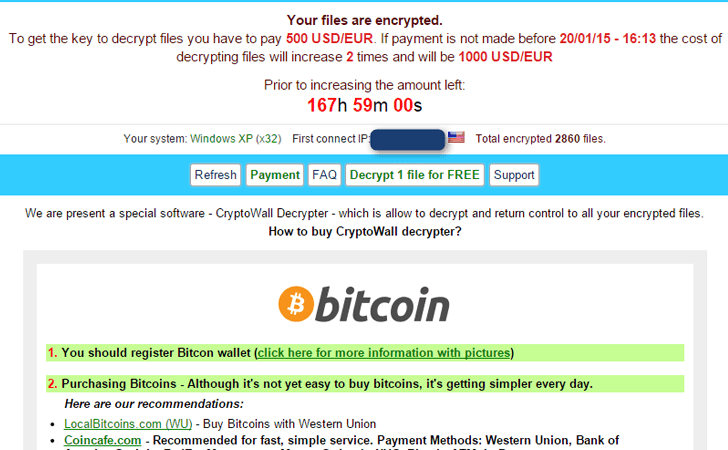
\includegraphics[width=\paperwidth]{cryptowall_ransom}
            };
        \end{tikzpicture}
    \end{frame}
}

\begin{frame}{malware}
    \begin{itemize}
    \item ``evil software''
    \item<2-> display a funny message
    \item<2-> send passwords/credit card numbers to criminals
    \item<2-> take pictures to send to criminals
    \item<2-> delete data
    \item<2-> hold data hostage
    \item<2-> insert/replace ads in webpages
    \item<2-> \ldots
    \end{itemize}
\end{frame}


\begin{frame}{viruses}
    \begin{itemize}
    \item malware that \myemph{inserts itself into another program}
    \item ``infects'' other programs when run
    \begin{itemize}
    \item usually modifies executables directly
    \end{itemize}
    \end{itemize}
\end{frame}

\begin{frame}{macro viruses}
    \begin{itemize}
    \item Word, Excel, other office software support \myemph{macros}
        \begin{itemize}
        \item scripts embedded in Word/Excel/etc. documents
        \end{itemize}
    \item viruses written in a \myemph{scripting language} 
        \begin{itemize}
        \item Visual Basic for Applications
        \end{itemize}
    \item spread to office documents, not executables
        \begin{itemize}
        \item easily spread in corporate environments
        \end{itemize}
    \item vendor reaction: macros disabled by default now
    \end{itemize}
\end{frame}

{ % all template changes are local to this group.
    \setbeamertemplate{navigation symbols}{}
    \begin{frame}[plain]
        \begin{tikzpicture}[remember picture,overlay]
            \node[at=(current page.center)] {
                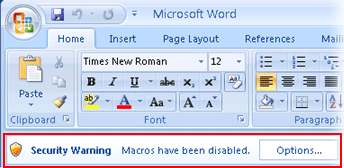
\includegraphics[width=\paperwidth]{msword-macro-warning}
            };
        \end{tikzpicture}
    \end{frame}
}

\begin{frame}{all viruses?}
    \begin{itemize}
    \item some sources call almost \myemph{all malware} \textit{virsues}
    \item or all self-propagating malware
    \vspace{.5cm}
    \item I won't --- but I will avoid testing you on this
    \item goal of hierarchy is knowing variety, not characterizing
    \end{itemize}
\end{frame}

\begin{frame}{worms}
    \begin{itemize}
    \item \myemph{independent program}
    \item usually ``blends in'' with system programs
    \item copies itself to other machines or USB keys, etc.
    \item sometimes configures systems to run it automatically
    \end{itemize}
\end{frame}

\begin{frame}{trojan (horse)s}
    \begin{itemize}
    \item \myemph{useful-looking} program that is malware:
        \begin{itemize}
        \item `cracked' version of commerical software
        \item fake anti-virus software
        \item or looks like useful PDF doc
        \item \ldots
        \end{itemize}
    \item maybe is (or not), but also does something evil
    \item common form for targeted attacks
    \end{itemize}
\end{frame}

\begin{frame}{potentially unwanted programs}
    \begin{itemize}
    \item unwanted software \myemph{bundled with wanted software}
    \item sometimes disclosed but in deceptive fine print
    \item sometimes considered malware, sometimes not
    \end{itemize}
\end{frame}

\begin{frame}{rootkit}
    \begin{itemize}
    \item root = full privileges 
        \begin{itemize}
        \item common name for Unix administrator account
        \end{itemize}
    \item rootkit = malware for \myemph{maintaining full control}
        \begin{itemize}
        \item thing that malware/attackers install
        \end{itemize}
    \item rootkits \myemph{evade removal, detection}
    \item e.g. program made invisible to ``task manager''/{\tt ps}
    \item e.g. reinstall malware if removed ``normally''
    \end{itemize}
\end{frame}

\begin{frame}{logic bomb}
    \begin{itemize}
    \item dormant malicious code
    \item e.g. from disgruntled employee before quitting
    \end{itemize}
\end{frame}

\section{Vulnerabilities and Exploits}

\begin{frame}{vulnerabilities}
    \begin{itemize}
    \item trojans: the vulnerability is the \myemph{user}
        \begin{itemize}
        \item and/or the user interface
        \end{itemize}
    \item otherwise?
    \item software \myemph{vulnerability}
    \vspace{.5cm}
    \item unintended program behavior \\ that can be used by an adversary
    \end{itemize}
\end{frame}

\begin{frame}{vulnerability example}
    \begin{itemize}
    \item website able to install software without prompting
    \item \myemph{not intended} behavior of web browser
    \end{itemize}
\end{frame}

\begin{frame}{software vulnerability classes (1)}
    \begin{itemize}
    \item \myemph{memory safety} bugs
        \begin{itemize}
        \item problems with pointers
        \item big topic in this course
        \end{itemize}
    \item ``injection'' bugs --- \myemph{type confusion}
        \begin{itemize}
        \item commands/SQL within name, label, etc.
        \end{itemize}
    \item integer overflow/underflow
    \item \ldots
    \end{itemize}
\end{frame}

\begin{frame}{software vulnerability classes (2)}
    \begin{itemize}
    \item not checking inputs/permissions
        \begin{itemize}
        \item \url{http://webserver.com/../../../../file-I-shouldn't-get.txt}
        \end{itemize}
    \item almost any 's ``undefined behavior'' in C/C++
    \item synchronization bugs: time-to-check to time-of-use
    \item \ldots{} more?
    \end{itemize}
\end{frame}

\begin{frame}{vulnerability versus exploit}
    \begin{itemize}
    \item exploit --- something that uses a vulnerability to do something
    \item proof-of-concept --- something = demonstration the exploit is there
        \begin{itemize}
        \item example: open a calculator program
        \end{itemize}
    \end{itemize}
\end{frame}

\begin{frame}{malware logistics: how?}
    \begin{itemize}
    \item what are they written in?
    \end{itemize}
\end{frame}

\begin{frame}{malware languages (1)}
    \begin{itemize}
    \item assembly language/machine code
        \begin{itemize}
        \item hand-coded or partially hand-coded
        \end{itemize}
    \vspace{.5cm}
    \item vulnerabilities deal with \myemph{machine code/memory layout}
    \item better for hiding malware from anti-malware tools
    \end{itemize}
\end{frame}

\begin{frame}{malware languages (2)}
    \begin{itemize}
    \item high-level scripting languages
        \begin{itemize}
        \item fast prototyping
        \item maintainability/efficiency not priority
        \item sometimes malicious scripts
        \item non-machine-code parts can use anything!
        \end{itemize}
    \item sometimes specialized ``toolkits'' \\
          example: Virus Construction Kit
    \end{itemize}
\end{frame}



\begin{frame}{malware spreading}
    \begin{itemize}
        \item vulnerable network-accessible services
        \item shared files/folders  
            \begin{itemize}
            \item autorun on USB sticks
            \item macros in Word/Excel/etc. files
            \end{itemize}
        \item email attachments
        \item websites + browser vulnerabilities
            \begin{itemize}
            \item JavaScript interpreter bugs
            \item Adobe Flash Player bugs
            \end{itemize}
    \end{itemize}
\end{frame}

\section{Defenses and Counter-Defenses}

\begin{frame}{malware defenses (1)}
    \begin{itemize}
        \item ``antivirus'' software:
        \vspace{.5cm}
        \item Windows Defender
        \item avast!
        \item Avira
        \item AVG
        \item McAfee
        \item \ldots
    \end{itemize}
\end{frame}

\begin{frame}{malware defenses (2)}
    \begin{itemize}
        \item app stores/etc. filtering (in theory)
            \begin{itemize}
            \item require developer registration
            \item blacklisting after the fact?
            \end{itemize}
        \item ``sandboxing'' policies
            \begin{itemize}
            \item don't let, e.g., game access your taxes
            \end{itemize}
    \end{itemize}
\end{frame}

\begin{frame}[plain]
    \begin{tikzpicture}[remember picture,overlay]
        \node[at=(current page.center)] {
            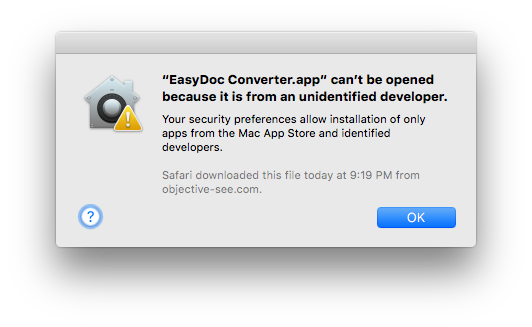
\includegraphics[width=\paperwidth]{app-denied-mac}
        };
    \end{tikzpicture}
\end{frame}

\begin{frame}[plain]
    \begin{tikzpicture}[remember picture,overlay]
        \node[at=(current page.center)] {
            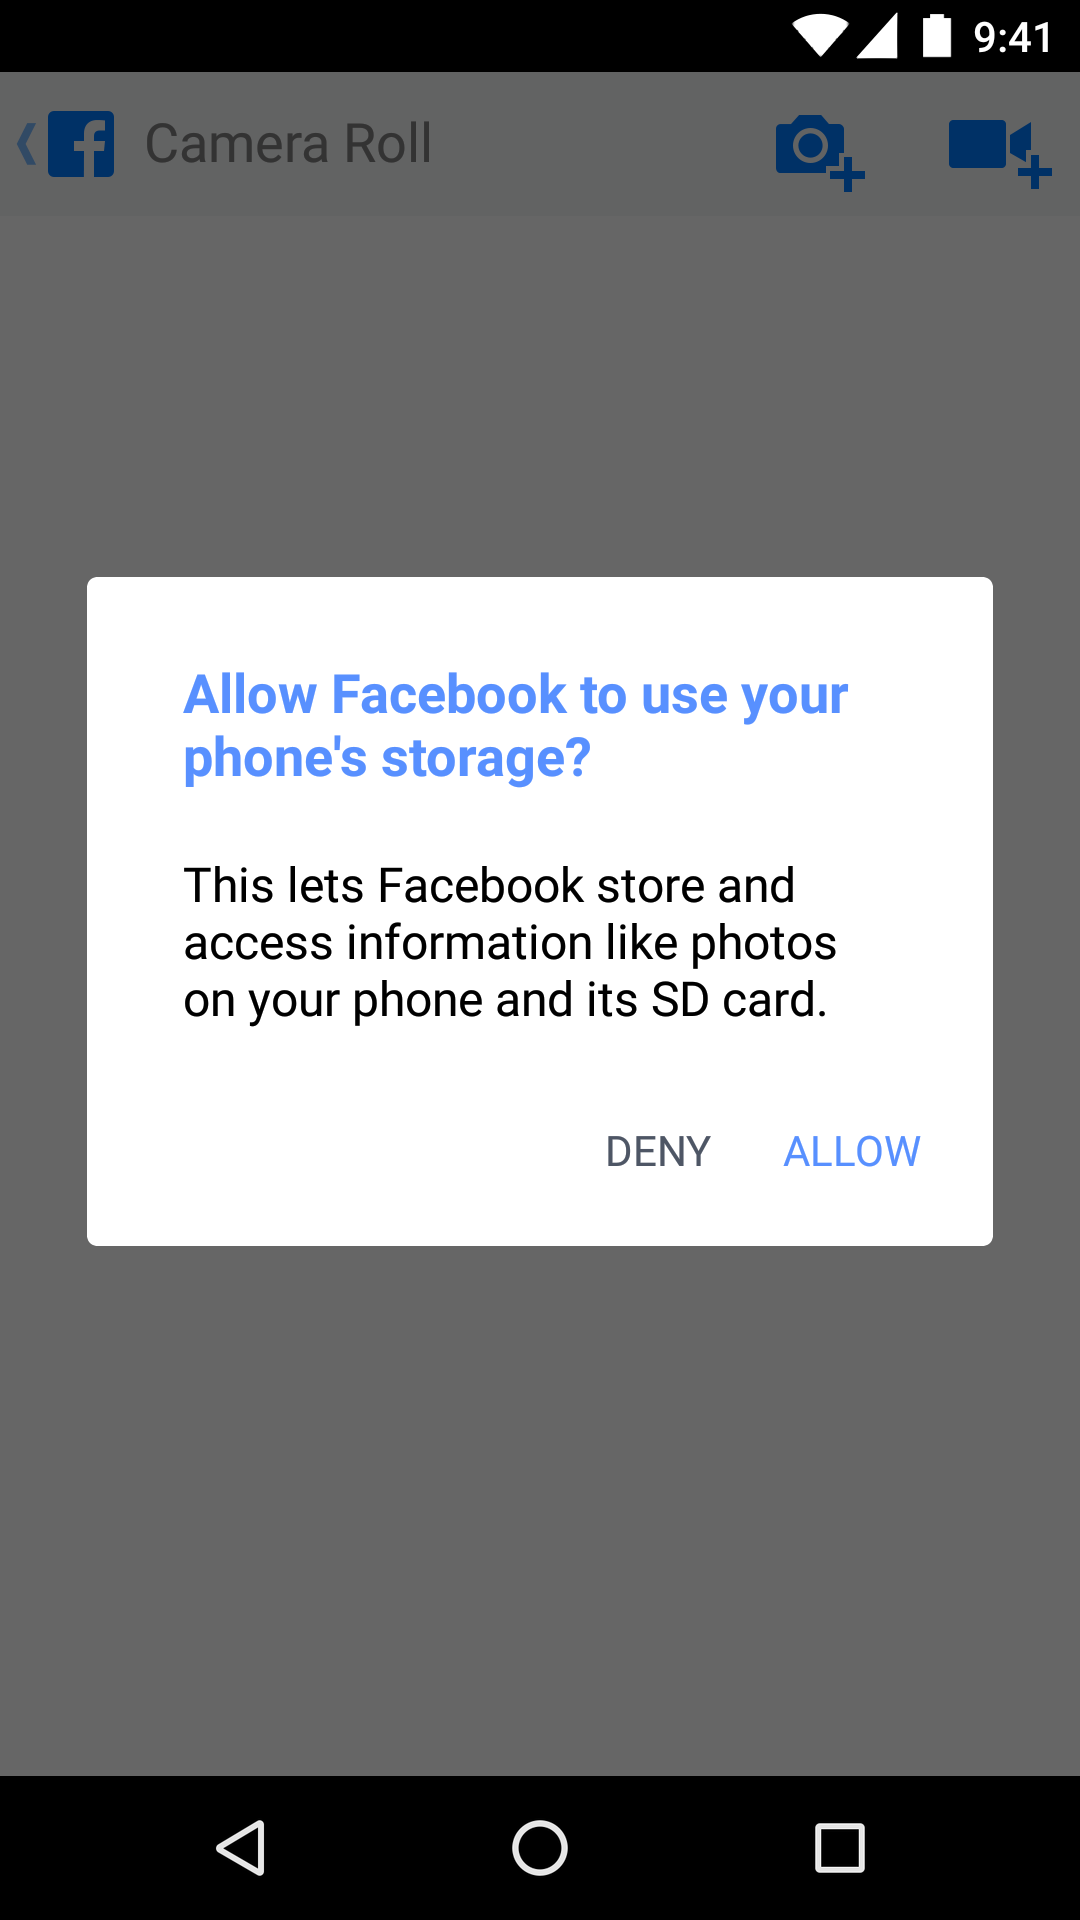
\includegraphics[width=\paperwidth]{facebook-perms-request}
        };
    \end{tikzpicture}
\end{frame}


\begin{frame}{malware defenses (3)}
    \begin{itemize}
        \item some email spam filters
        \item blacklists for web browsers
            \begin{itemize}
            \item Google Safe Browsing list (Chrome, Firefox)
            \item Microsoft SmartScreen (IE, Edge)
            \end{itemize}
    \end{itemize}
\end{frame}

\begin{frame}{malware counter-defenses}
    \begin{itemize}
    \item malware authors tries to make it hard-to-detect
    \item \myemph{obfuscation}:
        \begin{itemize}
        \item make code \myemph{harder to read}
        \item make code \myemph{different each time}
        \item \myemph{blend in} with normal files/applications/etc.
        \end{itemize}
    \end{itemize}
\end{frame}

\section{Some History}

\subsection{The Morris Worm}

\begin{frame}[plain]
    \begin{tikzpicture}[remember picture,overlay]
        \node[at=(current page.center)] {
            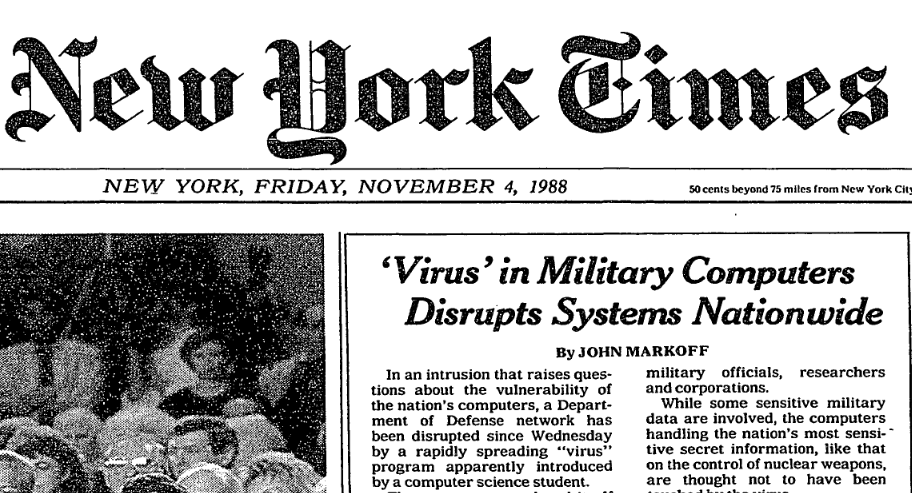
\includegraphics[width=\paperwidth]{nyt-head-virus}
        };
    \end{tikzpicture}
\end{frame}

\begin{frame}[plain]
    \begin{tikzpicture}[remember picture,overlay]
        \node[at=(current page.center)] {
            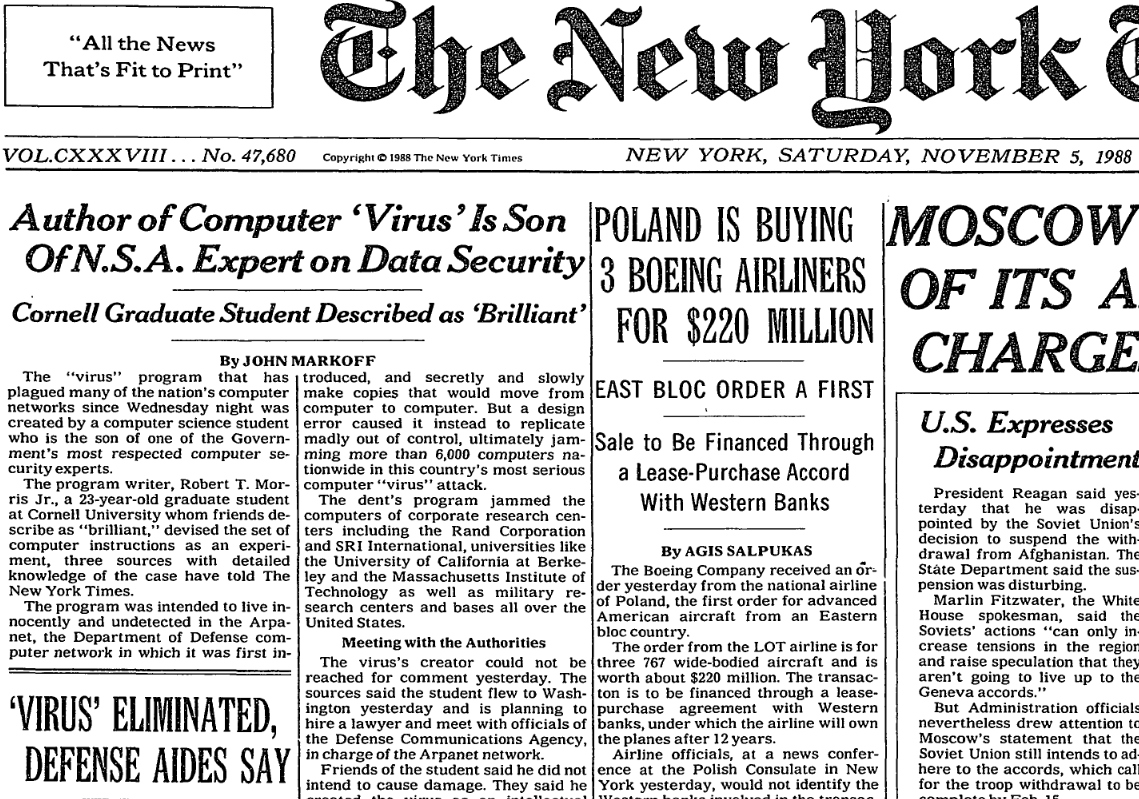
\includegraphics[width=\paperwidth]{nyt-head-morris}
        };
    \end{tikzpicture}
\end{frame}

\begin{frame}{Morris worm mechanisms}
\begin{itemize}
    \item used vulnerabilities in some versions of:
        \begin{itemize}
        \item mail servers ({\tt sendmail})
        \item user information servers ({\tt fingerd})
        \end{itemize}
    \item also spread using {\tt rsh}/{\tt rexec} (predecessor to ssh)
    \item hid by being called {\tt sh} (default shell)
    \item strings obscured slightly in binary
\end{itemize}
\imagecredit{Eichin and Rochlis, ``With Microscope and Tweezers: An Analysis of the Internet Virus of November 1998''}
\end{frame}

\begin{frame}{the early Internet}
    \begin{itemize}
    \item pretty homogeneous --- almost all Unix-like systems
    \item {\tt sendmail} was ``the'' email server to run
    \item most institutions vulnerable
    \end{itemize}
\end{frame}

\begin{frame}{Morris worm intent versus effect}
\begin{itemize}
\item code in viruses tried to avoid ``reinfecting'' machines
\item \ldots{} but not actually effective
\end{itemize}
\end{frame}

\subsection{Stuxnet}

\begin{frame}{Stuxnet}
    \begin{itemize}
        \item targeted Iranian nuclear enrichment facilities
        \item physically damaged centrifuges
        \item designed to spread via USB sticks
        \item publicly known 2010, deployed 2009
        \item US + Israel gov't developed
            \begin{itemize}
            \item according to press reports
            \end{itemize}
    \end{itemize}
\end{frame}

\subsection{Cryptolockers}

\begin{frame}{Ransomware}
    \begin{itemize}
        \item encrypt files, hold for ``ransom''
        \item decryption key stored only on attacker-controlled server
        \item possibly decrypt files if victim pays
        \vspace{.5cm}
        \item many millions in revenues 
        \begin{itemize}
            \item accurate numbers are hard to find
        \end{itemize}
    \end{itemize}
\end{frame}

\subsection{Adware}

\begin{frame}{ad injection (1)}
    \begin{itemize}
        \item internet advertising is big business
        \item \ldots{} but you need to pay websites to add ads?
        \item how about \myemph{modifying browser} to add/change ads
        \vspace{.5cm}
        \item mostly \myemph{bundled} with legitimate software
    \end{itemize}
\end{frame}


{ % all template changes are local to this group.
    \setbeamertemplate{navigation symbols}{}
    \begin{frame}[plain]
        \begin{tikzpicture}[remember picture,overlay]
            \node[at=(current page.center)] {
                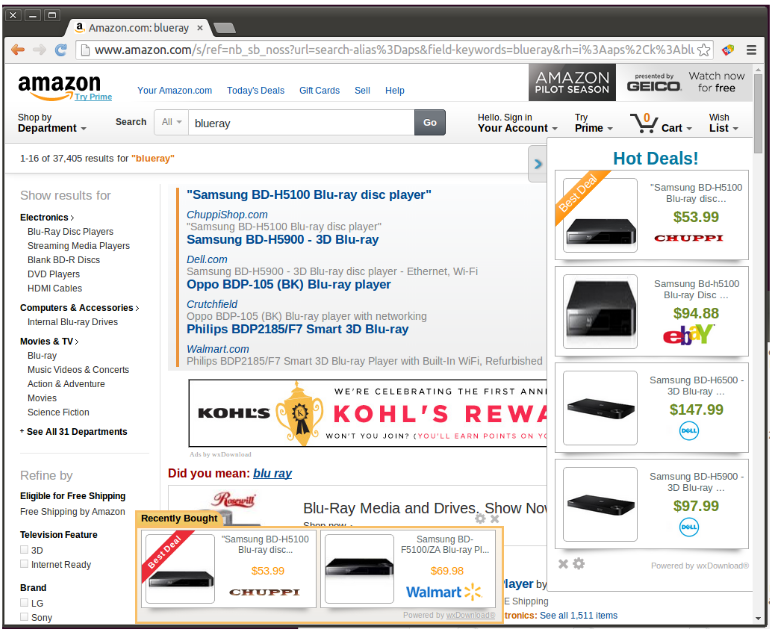
\includegraphics[height=0.96\paperheight]{ad-inject-amazon}
            };
        \end{tikzpicture}
    \imagecredit{From Thomas et al, ``Ad Injection at Scale: Assessing Deceptive Advertisement Modifications''}
    \end{frame}
}

\begin{frame}{ad injection (2)}
    \begin{itemize}
        \item 5\% of Google-accessing clients (2014)
        \item >90\% using code from VC-backed firm SuperFish:
        \vspace{.5cm}
            \item \$19.3 M in investment (CrunchBase)
            \item \$38M in revenue (Forbes, 2015)
            \item defunct after Lenovo root CA incident (2015)
            \item \ldots{} but founders reported started new, similar venture (JustVisual; according to TechCrunch)
    \end{itemize}
    \imagecredit{Adware prevalence: Thomas et al, ``Ad Injection at Scale: Assessing Deceptive Advertisement Modifications''}
\end{frame}

\subsection{Misc monetizations}

\begin{frame}{stealing banking credentials}
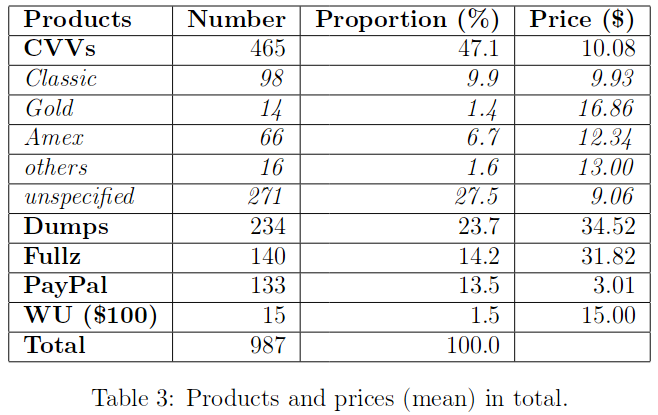
\includegraphics[width=\textwidth]{all-your-cards-tbl3}
\imagecredit{From Haslebacher et al, ``All Your Cards Are Belong To Us: Understanding Online Carding Forms'', arXiv preprint 1607.0017v1}
\end{frame}

\begin{frame}{web-camera blackmail}
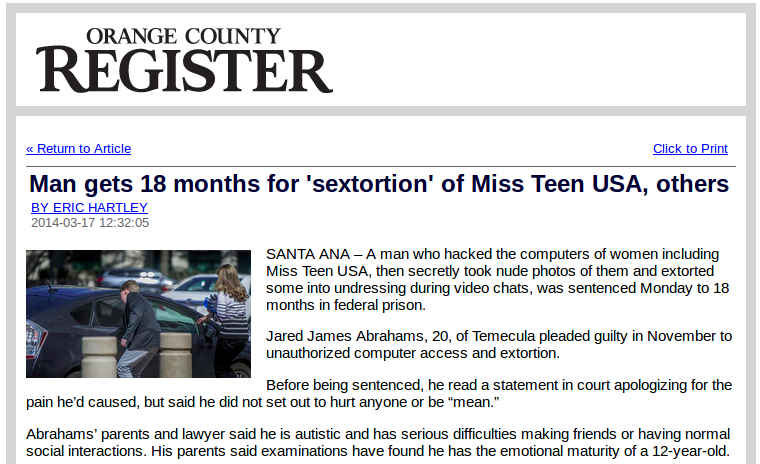
\includegraphics[width=\textwidth]{oc-sext-head}
\end{frame}

\begin{frame}{flooding websites}
    \begin{itemize}
    \item distributed denial of service
    \item example: October 2016 against DNS provider Dyn
        \begin{itemize}
        \item used by Twitter, GitHub, Amazon, \ldots, \ldots
        \end{itemize}
    \end{itemize}
\end{frame}

\begin{frame}{monetized DDoS}
    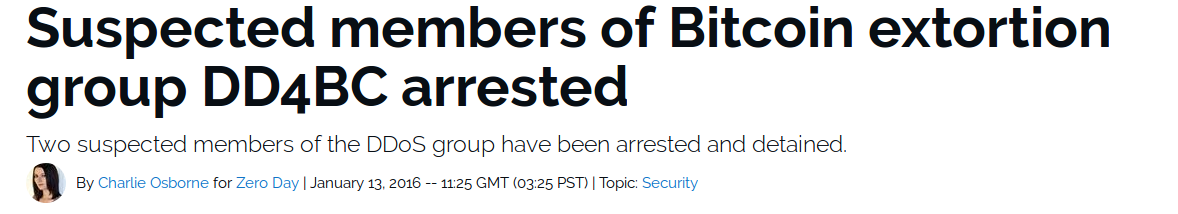
\includegraphics[width=\textwidth]{ddos-ext-head}  
\end{frame}

\begin{frame}{other motivations}
    \begin{itemize}
    \item ``cloud'' of hijacked machines for computation
    \item pride, vengeance (website defacement, etc.)
    \item \ldots
    \end{itemize}
\end{frame}

\begin{frame}{why talk about why/what?}
    \begin{itemize}
    \item doesn't change malware much
    \item (also, not a likely topic later in this course)
    \item \ldots but, attacking monetization is a real strategy
    \item attacker's willingness to spend?
    \end{itemize}
\end{frame}

\section{Logistics}

\begin{frame}{Website}
\begin{itemize}
    \item linked off Collab
    \item \url{https://www.cs.virginia.edu/~cr4bd/4630/S2017/}
    \item will include slides, assignments, lecture recordings
\end{itemize}
\end{frame}

\begin{frame}{lectures and attendance}
    \begin{itemize}
    \item I recommend coming to lecture
    \item I will not be taking attendance (except exams)
    \item Lectures will be recorded
    \end{itemize}
\end{frame}

\begin{frame}{Prerequisites}
\begin{itemize}
    \item \myemph{technically} CS 2150
    \item CS 3330 will be \myemph{very helpful}
\end{itemize}
\end{frame}

\begin{frame}{things from 3330 we care about}
    \begin{itemize}
    \item more review of \myemph{x86 assembly}
    \item \myemph{exceptions} and \myemph{virtual memory}
        \begin{itemize}
        \item (but probably not in much detail)
        \end{itemize}
    \end{itemize}
\end{frame}

\begin{frame}{Exams/Assignments}
\begin{itemize}
    \item many approx. one week assignments
    \vspace{.5cm}
    \item two midterms --- schedule on website
    \item one final
    \item can't make it? need accommodations? \myemph{tell us} ASAP!
\end{itemize}
\end{frame}

\begin{frame}{Textbook}
    \begin{itemize}
    \item no required textbook
    \item optional materials:
    % FIXME: picture
    \item Szor, \textit{The Art of Computer Virus Research and Defense}
    \item I can recommend more general books, too
    \end{itemize}
\end{frame}

\begin{frame}{TAs/Office Hours}
    \begin{itemize}
    \item TAs posted on website
    \item my office hours posted on website
    \item TA office hours will be posted
    \end{itemize}
\end{frame}

\begin{frame}{Piazza, etc.}
    \begin{itemize}
    \item Piazza --- linked of Collab
    \item TAs and I should be monitoring
    \vspace{.5cm}
    \item anonymous feedback on Collab
        \begin{itemize}
        \item (almost) always appreciated
        \end{itemize}
    \end{itemize}
\end{frame}

\begin{frame}{Misc. Policies}
    \begin{itemize}
    \item possibly exceptional circumstances? ask!
    \item there is a late policy
    \item assignments are \myemph{individual}
    \item don't cheat
    \item don't know if it's cheating? ask!
    \end{itemize}
\end{frame}

\section{On ethics/law}

\begin{frame}{On Ethics}
    \begin{itemize}
    \item don't use someone's computer without their permission
        \begin{itemize}
        \item or in excess of what they've permitted
        \end{itemize}
    \item don't assume it's just a harmless prank
        \begin{itemize}
        \item unintended (but likely) consequences
        \end{itemize}
    \item don't assume the system owner would give you permission
        \begin{itemize}
        \item if you're afraid to ask, it's not okay
        \end{itemize}
    \end{itemize}
\end{frame}

\begin{frame}{On Law}
    \begin{itemize}
    \item probably illegal (Federal and/or State crime):
    \vspace{.5cm}
    \item accessing computers without authorization
        \begin{itemize}
        \item even if nothing is done with the access
        \end{itemize}
    \item deliberately overloading a service
    \item ``backhacking'' into a malware operator's machine
    \item deploying a worm that patches security holes
    \end{itemize}
\end{frame}

\begin{frame}
    \begin{itemize}
    \item ethics pledge --- please \myemph{read} and sign
        \begin{itemize}
        \item on website, or I have copies
        \end{itemize}
    \item questions about ethics?
    \end{itemize}
\end{frame}

\section{VM assignment}

\begin{frame}{VM}
    \begin{itemize}
    \item homework assignments
    \item first assignment --- get an appropriate VM working
    \end{itemize}
\end{frame}

\begin{frame}{VM environment}
    \begin{itemize}
    \item \textbf{64-bit} Ubuntu 16.04 LTS
    \item some assignments will \myemph{require exactly this}
    \item (not some other Linux, not 32-bit)
    \end{itemize}
\end{frame}

\begin{frame}{VM problems?}
    \begin{itemize}
    \item \textbf{tiny} possibility your machine \textbf{can't} run 64-bit VM
    \item (\textbf{no} CPU support --- not ``it's hard to setup'')
    \vspace{.5cm}
    \item we can find alternative solutions for you
    \item talk to us!
    \end{itemize}
\end{frame}

\begin{frame}{related assignment}
    \begin{itemize}
    \item due 27 Jan (week from Friday) at 5PM
    \item assignment on website
    \item submission on Collab
    \end{itemize}
\end{frame}

\begin{frame}{next time: on VMs}
    \begin{itemize}
    \item virtual machines --- what, why, how
    \item virtual machines and malware
    \end{itemize}
\end{frame}

\section{Semester Outline}

\begin{frame}{topics outline}
    \begin{itemize}
    \item prerequisite: assembly review
    \item malware history
    \item cat-and-mouse: anti-malware
    \item software vulnerabilities
    \begin{itemize}
        \item memory management related
    \end{itemize}
    \item bonus topics: 
        \begin{itemize}
        \item ``safe'' languages
        \item web browser security
        \end{itemize}
    \end{itemize}
\end{frame}

\section{Conclusion}

\begin{frame}{Conclusion}
    \begin{itemize}
    \item malware: ``evil'' software
        \begin{itemize}
        \item originally --- thrill? proof of concept?
        \item commonly --- monetary motives
        \end{itemize}
    \item vulnerabilities:
        \begin{itemize}
        \item exploitable unintended program behavior
        \end{itemize}
    \end{itemize}
\end{frame}
